
\begin{figure}[ht]
	\begin{center}
		\caption{Firm Payoff as a Function of Public Float  }\label{fig:payoff}
		\begin{subfigure}{0.48\textwidth}
			\begin{tikzpicture}
				
				\draw[thick,<->] (0,5) node[above]{Payoff}--(0,0)--(6,0) node[right]{Equity};
				
				\def\qs{3}
				\def\qd{2}
				
				\draw[thick,dashed] (\qs,0) node[below]{$z$}--(\qs,5) ;
				
				
				\begin{scope}
					\clip (\qs-2.5,1) rectangle (\qd,5);
					\draw[thick] (\qs-2.5,1)..controls (\qs,6) ..(\qs+2.5,1);
				\end{scope}
				\draw[thick,gray] (\qs-2.5,1)..controls (\qs,6) ..(\qs+2.5,1);	
				\draw (\qs,5) node[above]{$-\Phi(e;z)$};
				
				
			\end{tikzpicture}
			
			\caption{No regulatory threshold }\label{fig:no_threshold}
		\end{subfigure}
		\hspace*{\fill}  % spread out the first and second subfigures
		\begin{subfigure}{0.48\textwidth}
			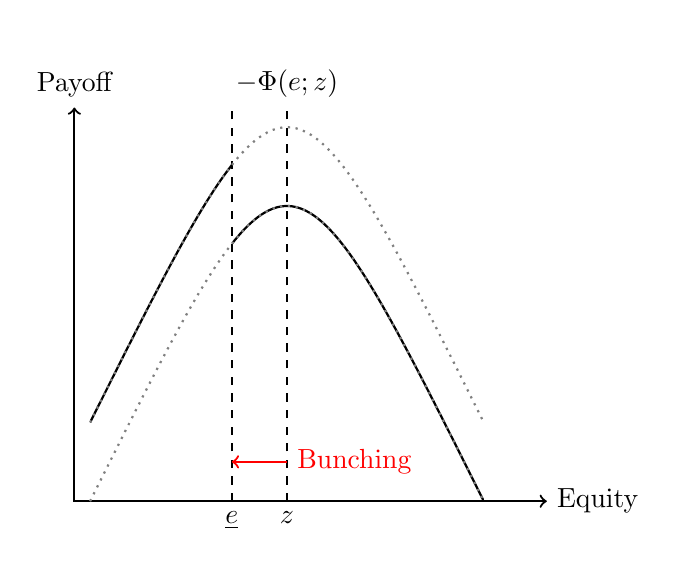
\begin{tikzpicture}
				
				\draw[thick,<->] (0,5) node[above]{Payoff}--(0,0)--(6,0) node[right]{Equity};
				
				\def\qs{2.7}
				\def\qd{2}
				
				\draw[thick,dashed] (\qs,0) node[below]{$z$}--(\qs,5) ;
				\draw[thick,dashed] (\qd,0) node[below]{$\underline{e}$}--(\qd,5) ;
				
				
				\begin{scope}
					\clip (\qs-2.5,1) rectangle (\qd,5);
					\draw[thick] (\qs-2.5,1)..controls (\qs,6) ..(\qs+2.5,1);
				\end{scope}
				\draw[thick,dotted,gray] (\qs-2.5,1)..controls (\qs,6) ..(\qs+2.5,1);	
				\draw (\qs,5) node[above]{$-\Phi(e;z)$};
				
				
				\def\y{-1}
				\begin{scope}
					\clip (\qs+2.5,1+\y) rectangle (\qd,5+\y);
					\draw[thick] (\qs-2.5,1+\y)..controls (\qs,6+\y) ..(\qs+2.5,1+\y);
				\end{scope}
				\draw[thick,dotted,gray] (\qs-2.5,1+\y)..controls (\qs,6+\y) ..(\qs+2.5,1+\y);	
				
				\draw[thick,red,->] (\qs,.5) node[above,right]{Bunching} --(\qd,.5);		
			\end{tikzpicture}
			\caption{Bunching at regulatory threshold }\label{fig:bunching_at_threshold}
		\end{subfigure}
		\medskip
		\begin{subfigure}{0.48\textwidth}
			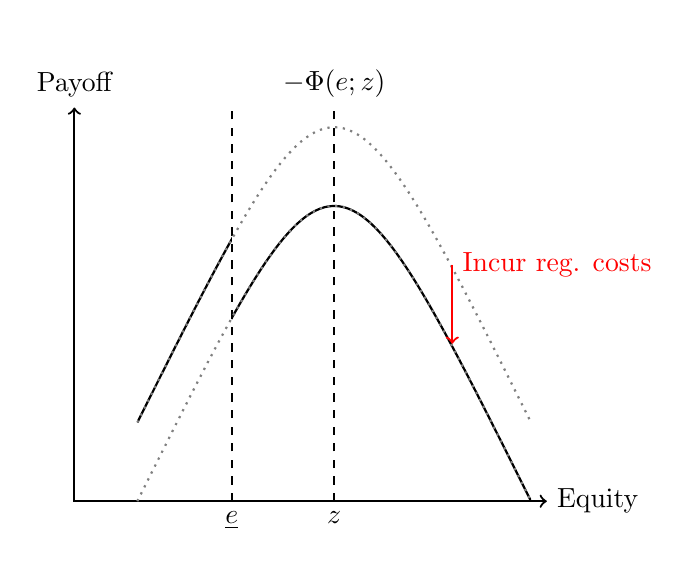
\begin{tikzpicture}
				
				\draw[thick,<->] (0,5) node[above]{Payoff}--(0,0)--(6,0) node[right]{Equity};
				
				\def\qs{3.3}
				\def\qd{2}
				
				
				\draw[thick,dashed] (\qs,0) node[below]{$z$}--(\qs,5) ;
				\draw[thick,dashed] (\qd,0) node[below]{$\underline{e}$}--(\qd,5) ;
				
				
				\begin{scope}
					\clip (\qs-2.5,1) rectangle (\qd,5);
					\draw[thick] (\qs-2.5,1)..controls (\qs,6) ..(\qs+2.5,1);
				\end{scope}
				\draw[thick,dotted,gray] (\qs-2.5,1)..controls (\qs,6) ..(\qs+2.5,1);	
				\draw (\qs,5) node[above]{$-\Phi(e;z)$};
				
				
				\def\y{-1}
				\begin{scope}
					\clip (\qs+2.5,1+\y) rectangle (\qd,5+\y);
					\draw[thick] (\qs-2.5,1+\y)..controls (\qs,6+\y) ..(\qs+2.5,1+\y);
				\end{scope}
				\draw[thick,dotted,gray] (\qs-2.5,1+\y)..controls (\qs,6+\y) ..(\qs+2.5,1+\y);	
				
				\draw[thick,red,->] (\qs+1.5,3) node[above,right]{Incur reg. costs} --(\qs+1.5,2);	
			\end{tikzpicture}
			\caption{Not bunching}\label{fig:not_bunching}
		\end{subfigure}
		\hspace*{\fill}  % spread out the first and second subfigures
		\begin{subfigure}{0.48\textwidth}
			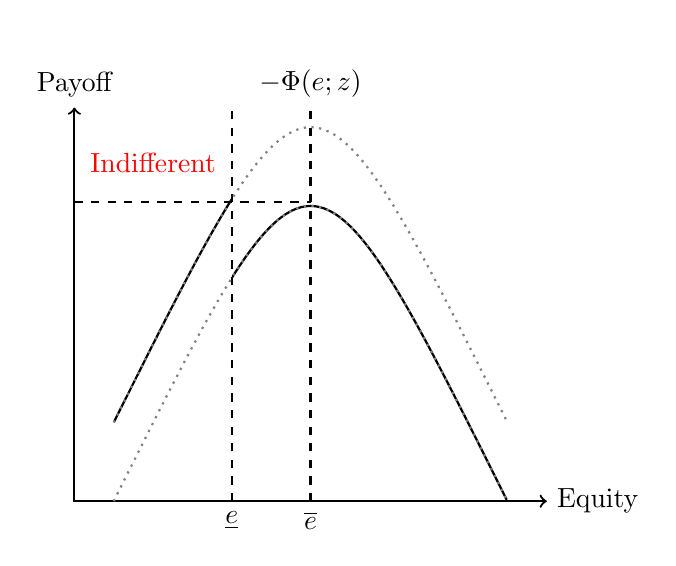
\begin{tikzpicture}
				
				\draw[thick,<->] (0,5) node[above]{Payoff}--(0,0)--(6,0) node[right]{Equity};
				
				\def\qs{3}
				\def\qd{2}
				
				
				\draw[thick,dashed] (\qd,0) node[below]{$\underline{e}$}--(\qd,5) ;
				
				\draw[thick,dashed] (\qs,0) node[below]{$\overline{e}$}--(\qs,5) ;
				
				
				\begin{scope}
					\clip (\qs-2.5,1) rectangle (\qd,5);
					\draw[thick] (\qs-2.5,1)..controls (\qs,6) ..(\qs+2.5,1);
				\end{scope}
				\draw[thick,dotted,gray] (\qs-2.5,1)..controls (\qs,6) ..(\qs+2.5,1);	
				\draw (\qs,5) node[above]{$-\Phi(e;z)$};
				
				
				\def\y{-1}
				\begin{scope}
					\clip (\qs+2.5,1+\y) rectangle (\qd,5+\y);
					\draw[thick] (\qs-2.5,1+\y)..controls (\qs,6+\y) ..(\qs+2.5,1+\y);
				\end{scope}
				\draw[thick,dotted,gray] (\qs-2.5,1+\y)..controls (\qs,6+\y) ..(\qs+2.5,1+\y);	
				\draw[thick,dashed] (0,3.8)--(\qs,3.8)node [red,midway,yshift=.5cm,xshift=-.5cm] {Indifferent}; ;	
			\end{tikzpicture}
			
			\caption{Marginal buncher}\label{fig:marginal_buncher}
		\end{subfigure}
		
		\label{fig:bunching_explained}
	\end{center}
	{\small{}This figure illustrates the shape of a firm's payoff as a function of the public float $e$. Panel (a) illustrates a concave payoff function in the absence of a regulatory threshold. Panel (b) shows a new payoff function when a regulatory threshold is introduced at  $\underline{e}$. The discontinuity in the payoff induces firms whose public float was somewhat above the threshold to bunch. Panel (c) shows a firm whose undistorted optimal float is way above the regulatory threshold and therefore chooses not to bunch. Panel (d) shows a payoff function for the marginal bunching firm who is indifferent between bunching and not bunching. } {\small\par}
\end{figure}